\documentclass[12pt,a4paper]{article}
%\usepackage[cm]{fullpage}
\usepackage[margin=0.5in]{geometry}
\usepackage{graphicx}
\usepackage{floatrow}
\usepackage{authblk} 
\usepackage{etoolbox}
\usepackage{lmodern}

\date{}
\pagestyle{empty}

\begin{document}

\makeatletter
\patchcmd{\@maketitle}{\LARGE \@title}{\fontsize{18}{19.2}\selectfont\@title}{}{}
\makeatother
\renewcommand\Authfont{\fontsize{12}{14.4}\selectfont}
\renewcommand\Affilfont{\fontsize{10}{10.8}\selectfont}


\title{Sampling in a hierarchical model of images reproduces top-down effects in visual perception}
\author{Mih\'aly B\'anyai, Gerg\H{o} Orb\'an}
\affil{Computational Systems Neuroscience Lab, Wigner Research Centre for Physics, Budapest, Hungary}
\maketitle
\thispagestyle{empty}

Sensory perception can be understood as inference of latent causes underlying stimuli. This requires animals to learn the statistics of the environment in terms of a generative model with latent variables corresponding to features with hierarchical organisation, which is characteristic of efficient probabilistic models (Hinton, 2006). While layers of probabilistic image models map intuitively to the hierarchical structure of the ventral stream, details of the correspondence have remained elusive.

Mean activity at the lowest level of visual hierarchy, V1 simple cells, are well covered by linear filters adapted to the statistics of natural scenes (Olshausen, 1996) and by a more elaborate model describing interactions between filters (Schwartz, 2001). Effects of top-down interactions on mean responses have been formalised in terms of covariance components of latent variables (Karklin, 2008). However, thorough understanding requires that other aspects of the rich response statistics can also be linked to computational principles.

A computationally appealing and neurally feasible method to perform Bayesian inference is the construction of stochastic samples (Lee, 2003). Sampling establishes a link between the neural response distribution and probability distributions in Bayesian models. We explore sampling in a hierarchical model of vision and its consequences on neural response statistics in V1. 

We have built a hierarchical model of the visual system that bears similarities with the covariance model of Karklin, and used sampling to perform Bayesian inference in it. Activity of model neurons were regarded as samples from the posterior distribution resulting from inference. Top-down effects in the visual hierarchy are particularly noticeable in the phenomenon of illusory contours, thus we used synthetic images with the model to predict the neural response to such stimuli. The sampling algorithm reproduces the magnitude ratio and temporal evolution of neural responses to real and illusory contours, measured from V1 and V2 (Lee, 2001). 

\vspace{5mm}

{\bf Inference by sampling in the covariance component model.} We defined two layers of latent variables that control the distribution of observed pixels (see Fig. 1A). Higher-level units ($g$) serve as coefficients for additive mixing of the $K$ components of the Gaussian covariance of the lower-level units ($v$). $P(v | g) = \mathcal{N}(v;0,C_v)$, where $C_v = \sum_{j=1}^K g_jC_j$. In turn, $v$-units define the Gaussian mean of pixels ($x$) through a set of linear filters ($A$) (for a similar formulation see Karklin \& Lewicki, 2008). The pixel statistics also depend on a scalar contrast variable ($z$) and an independent observation noise. $P(x|v,z) = \mathcal{N}(zAv,\sigma_x I)$. Prior densities of $g$ and $z$ are defined as fixed-parameter Gamma distributions, allowing us to produce synthetic data by defining all model parameters and conducting ancestral sampling. Bayesian inference in the model can be implemented by sampling the posterior distributions, which procedure is hypothesised to correspond to cortical representation of uncertainty (Orb\'an, 2008). MCMC samples are obtained using a Gibbs sampling scheme cycling over the conditional posteriors of the three variable groups $v$,$g$ and $z$. 

\begin{eqnarray}
p(v \mid x,g,z) = \mathcal{N}\left(v; \frac{z}{ \sigma_x} \left( \frac{z^2}{ \sigma_x} A^T A + C_v^{-1}\right)^{-1} A^T x, \left(\frac{z^2}{\sigma_x} A^T A + C_v^{-1}\right)^{-1}\right) \\
\log p(g \mid X,V) \sim -\frac{1}{2} \left[\log(\det(C_v)) + v^T C_v^{-1} v \right] + (\alpha-1) + \log p(g) \\
\log p(z \mid X,V) \sim -\frac{1}{2} \left[ D_x\log(\sigma_x) + \frac{1}{\sigma_x}  (x - zAv)^T (x - zAv)\right] + \log p(z)
\end{eqnarray}
%
The conditional posteriors of g and z need to be sampled by MCMC steps themselves. The acquired samples can also be used to learn the elements of the covariance component matrices from data in an unsupervised manner by calculating the expectation of the complete-data log-likelihood of the model, and conducting gradient descent on the resulting expression as a generalised expectation-maximisation scheme. This provides a candidate procedure to model the data-driven acquisition of covariance components characteristic to natural stimuli, which we validated on synthetic datasets. The fact that the model can learn multiple correlational contexts and infer their composition contributing to an image patch extends the range of phenomena that can be modelled by it relative to single-covariance models such as Gaussian Scale Mixtures (Schwartz \& Simoncelli, 2001). Instead of relying only on the second-order statistics of the filter coefficients, our model uses higher-order statistics represented by the covariance components, thus making it possible to learn and perceive multiple spatially overlapping covariance structures without having them average out or lump together. Such learned covariance structures may also be understood as formalisations Gestalt effects observed in behavioural measurements of perception.

{\bf Prediction of responses to illusory contours.} Neurons in the primary visual cortex are sensitive to illusory contours (IC) defined by contextual cues. However, the timing of such responses is delayed compared to responses to edge-defined contours by approximately 55 ms. Furthermore, appearance of IC-evoked responses in the secondary visual cortex (V2) precedes that in V1, suggesting a top-down direction of information flow (see Lee \& Nguyen, 2001 and Fig. 1D). To reproduce this effect, we constructed synthetic stimuli consisting of line segments, from which we occluded the receptive field of a selected V1 neuron (see Fig. 1B). We defined a model that consisted of several covariance components reflecting such line segments and a set of Gabor filters as projective fields of $v$-units. We ran Gibbs sampling to obtain time series for cell activations (Fig. 1C). As the switching on of the $g$-unit corresponding to the line segment activated the $v$-unit in a top-down manner, samples trajectories reproduced the measured magnitude ratio and timing of IC responses (Fig.1C). As detection of continuous features despite of occlusion is crucial for object recognition, the presented functionality may serve as a useful second step in the hierarchical processing of images. The sampling procedure generates testable predictions about the trial-to-trial variability and noise correlation of V1 neurons that may be compared to electrophysiological measurements from experiments with controlled Gestalt effects.

\begin{figure}[h]
\floatbox[{\capbeside\thisfloatsetup{capbesideposition={right,top},capbesidewidth=6cm}}]{figure}[\FBwidth]
{\caption{{\bf A.} Outline of the covariance component model with the three latent variable groups. {\bf B.} Two overlapping covariance components of the test model on the top, and the stimulus together with the percept of the model formed by posterior samples. {\bf C.} Time evolution of samples from the V1 cells with receptive fields at stimulated, occluded and other stimulus part and the G-cell with the left covariance component. Red line indicates the beginning and the end of stimulus presentation. {\bf D.} Reproduction of V1 responses to IC and line stimuli created by Kanizsa triangles from Lee \& Nguyen, 2001.
}\label{fig:test}}
{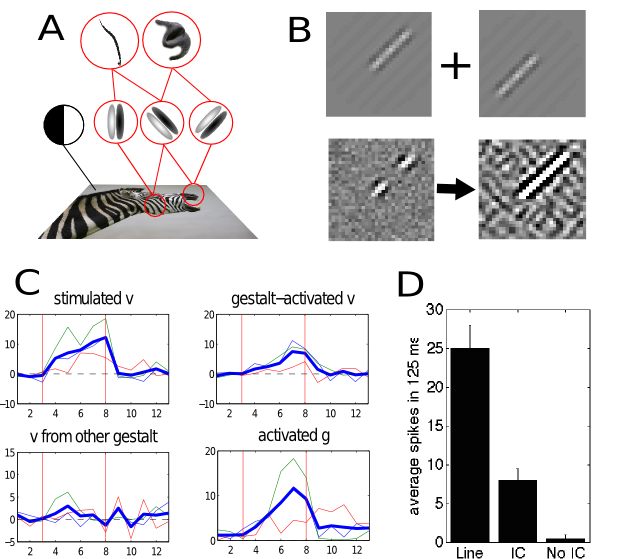
\includegraphics[width=10cm]{cosyne_figure.png}}
\end{figure}


\end{document}
